% =============================================================================
% CHAPTER 4: Results and Evaluation
% =============================================================================
% SPDX-FileCopyrightText: 2026 Frank Langbein <frank@langbein.org>
% SPDX-License-Identifier: LPPL-1.3c
%
% Suggested sections: Setup (or Evaluation setup / Experimental setup); Results;
% Discussion (or Evaluation and discussion); Limitations. Optional: Ablation
% studies (AI/ML); Comparison with baselines; Threats to validity. Describe how
% you demonstrated the system or hypothesis; include critical tests/experiments;
% critically appraise strengths and weaknesses.
% =============================================================================

This chapter presents the results and evaluates them. Describe how the solution was demonstrated, include test or experimental results, and critically appraise strengths and weaknesses.

%\lipsum[25-26]

\section{Setup}\label{sec:setup}
% Evaluation setup: data, metrics, baselines, how experiments or tests were run.
% Optional subsections: environment, hyperparameters, evaluation protocol.

%\lipsum[27-28]

\section{Results}\label{sec:results}
% Main findings: present tables and figures; summarise key outcomes. Optional
% subsections: by research question, by dataset, or by metric.

\subsection{Structural Consistency}\label{sec:node-counts}

\begin{table}[H]
\centering
\caption{Comparison of Scene Graph Node Statistics across Methods}
\label{tab:node_stats_transposed}
\begin{tabular}{l | ccc | ccc | ccc}
\toprule
\textbf{Method} & \multicolumn{3}{c|}{\textbf{Total Nodes}} & \multicolumn{3}{c|}{\textbf{Room Nodes}} & \multicolumn{3}{c}{\textbf{Object Nodes}} \\
 & Avg & Std & CV & Avg & Std & CV & Avg & Std & CV \\
\midrule
S-Graphs+ & 95.40 & 0.89 & 0.01 & 1.00 & 0.00 & 0.00 & --- & --- & --- \\
Hydra     & 1205.0 & 15.40 & 0.01 & 3.00 & 1.67 & 0.56 & 65.40 & 3.26 & 0.05 \\
Clio      & 1972.0 & 25.67 & 0.01 & 12.80 & 2.32 & 0.18 & 2.20 & 0.40 & 0.18 \\
\bottomrule
\end{tabular}
\end{table}

\subsection{Room Segmentation}\label{sec:rooms}

\begin{table}[H]
\centering
\caption{Room Recognition Comparison: Method Performance across Metrics. \textbf{Best results in bold.}}
\label{tab:room_recognition_transposed}
\begin{tabular}{l | ccc | ccc | ccc}
\toprule
\textbf{Method} & \multicolumn{3}{c|}{\textbf{Recall}} & \multicolumn{3}{c|}{\textbf{Precision}} & \multicolumn{3}{c}{\textbf{F1-Score}} \\
 & Avg & Std & CV & Avg & Std & CV & Avg & Std & CV \\
\midrule
S-Graphs+ & 0.67 & 0.00 & 0.00 & 0.56 & 0.03 & 0.06 & \textbf{0.61} & 0.02 & 0.03 \\
Hydra     & 0.43 & 0.25 & 0.58 & \textbf{0.90} & 0.15 & 0.17 & 0.55 & 0.21 & 0.39 \\
Clio      & \textbf{0.93} & 0.09 & 0.10 & 0.45 & 0.06 & 0.14 & 0.60 & 0.06 & 0.10 \\
\bottomrule
\end{tabular}
\end{table}

\subsection{Object Detection}\label{sec:object}

\begin{table}[H]
\centering
\caption{Spatial Accuracy Comparison: Method Performance across Drift and MED. \textbf{Best results in bold.}}
\label{tab:spatial_stats_transposed}
\begin{tabular}{l | ccc | ccc}
\toprule
\textbf{Method} & \multicolumn{3}{c|}{\textbf{Drift (m)}} & \multicolumn{3}{c}{\textbf{MED (m)}} \\
 & Avg & Std & CV & Avg & Std & CV \\
\midrule
Hydra     & \textbf{0.16} & 0.72 & 4.50 & \textbf{0.71} & 0.69 & 0.97 \\
Clio      & 2.18 & 2.74 & 1.25 & 3.36 & 0.53 & 0.17 \\
\bottomrule
\end{tabular}
\end{table}

\subsection{Semantic Accuracy}\label{sec:labels}

\begin{table}[H]
\centering
\caption{Comparison of Label Distribution across Methods}
\label{tab:label_dist_transposed}
\begin{tabular}{l | ccc}
\toprule
\textbf{Method} & \multicolumn{3}{c}{\textbf{All Labels}} \\
 & Avg & Std & CV \\
\midrule
Hydra & \textbf{5.95} & 0.54 & 0.21 \\
Clio  & 2.20 & 0.45 & 0.20 \\
\bottomrule
\end{tabular}
\end{table}

\begin{figure}[h]
    \centering
    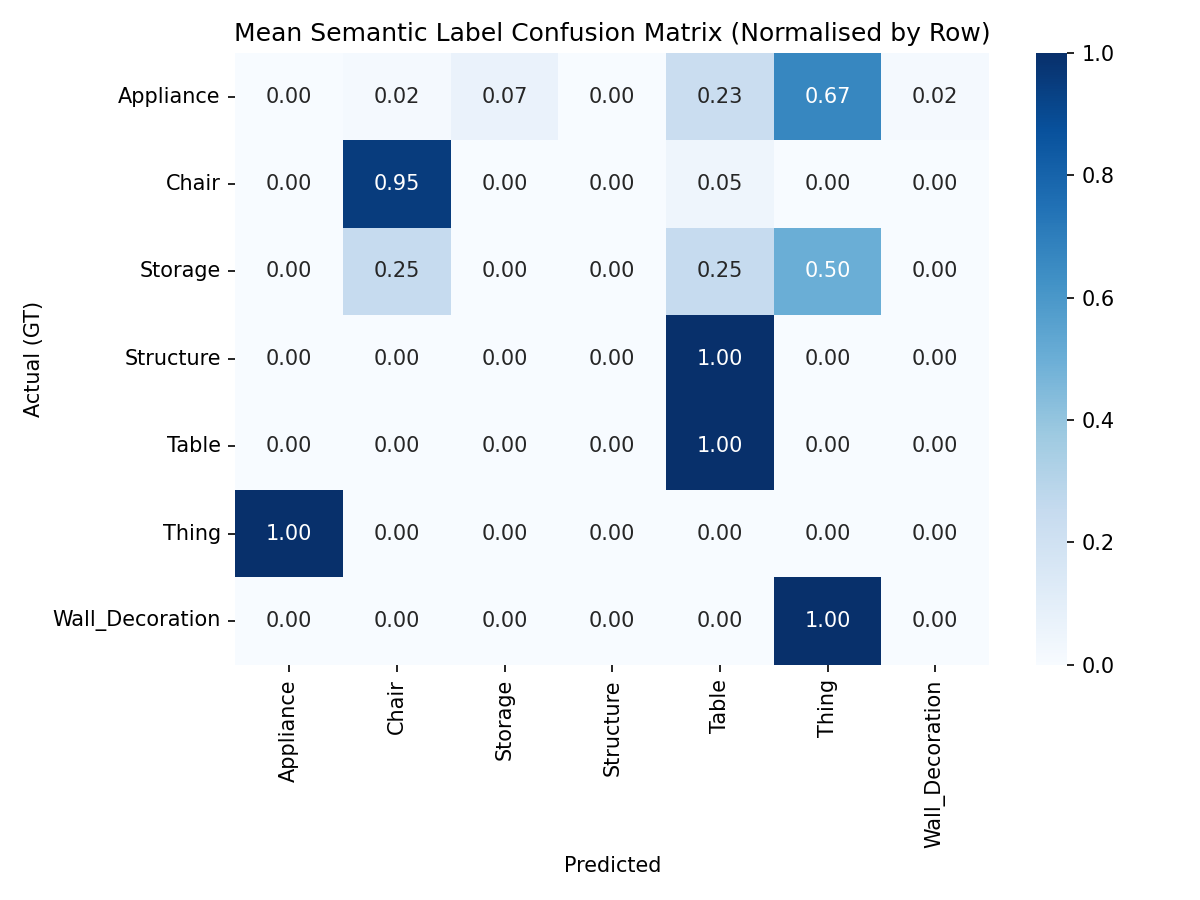
\includegraphics[width=0.5\textwidth]{figures/confusion_matrix_mean_norm.png}
    \caption{Normalised Confusion Matrix of Hydra Labels vs Ground Truth Labels}
    \label{fig:cmatrix}
\end{figure}

\subsection{Practicality}\label{sec:timing}

\begin{table}[H]
\centering
\caption{System Timing Comparison across Stages (Seconds). \textbf{Best results in bold.}}
\label{tab:timing_transposed}
\begin{tabular}{l | ccc | ccc | c}
\toprule
\textbf{Method} & \multicolumn{3}{c|}{\textbf{Frontend}} & \multicolumn{3}{c|}{\textbf{Backend}} & \textbf{Total (Avg)} \\
 & Avg & Std & CV & Avg & Std & CV & \\
\midrule
Hydra    & 0.105 & 0.002 & 0.020 & 0.058 & 0.001 & 0.018 & 0.162 \\
Clio     & \textbf{0.082} & 0.001 & 0.012 & 0.070 & 0.002 & 0.031 & \textbf{0.152} \\
S-Graphs+ & --- & --- & --- & \textbf{0.019} & 0.002 & 0.086 & --- \\
\bottomrule
\end{tabular}
\end{table}

%\lipsum[29-30]

\section{Real-World Results}\label{sec:r-w-results}

\section{Discussion}\label{sec:discussion}
% Critical appraisal: strengths, weaknesses, methodology choices; comparison
% with prior work. Optional: ablation analysis, sensitivity analysis.

%\lipsum[31-32]

\section{Limitations}\label{sec:limitations}
% Limitations, threats to validity, and suggested further tests if not all done.

%\lipsum[33-34]
